% ============================================================================
% PDF2TeX Module - Software Architecture Document
% ============================================================================
% Version: 1.0.0
% Date: January 2026
% Page Size: A3 Landscape for optimal diagram visibility
% ============================================================================

\documentclass[11pt]{article}

% ============================================================================
% PACKAGES
% ============================================================================
\usepackage[utf8]{inputenc}
\usepackage[T1]{fontenc}
\usepackage{lmodern}
\usepackage[a3paper,landscape,margin=2.5cm]{geometry}
\setlength{\headheight}{14pt}
\addtolength{\topmargin}{-2pt}
\usepackage{tikz}
\usepackage{xcolor}
\usepackage{graphicx}
\usepackage{float}
\usepackage{booktabs}
\usepackage{array}
\usepackage{longtable}
\usepackage{multirow}
\usepackage{enumitem}
\usepackage{hyperref}
\usepackage{fancyhdr}
\usepackage{titlesec}
\usepackage{tocloft}
\usepackage{caption}
\usepackage{subcaption}
\usepackage{multicol}
\usepackage{parskip}

% TikZ Libraries
\usetikzlibrary{
    shapes.geometric,
    shapes.misc,
    shapes.symbols,
    arrows.meta,
    positioning,
    calc,
    fit,
    backgrounds,
    decorations.pathreplacing,
    calligraphy,
    shadows.blur
}

% ============================================================================
% COLOR DEFINITIONS
% ============================================================================
\definecolor{primary}{HTML}{2563EB}       % Blue
\definecolor{secondary}{HTML}{7C3AED}     % Purple
\definecolor{accent}{HTML}{059669}        % Green
\definecolor{warning}{HTML}{D97706}       % Orange
\definecolor{danger}{HTML}{DC2626}        % Red
\definecolor{neutral}{HTML}{6B7280}       % Gray
\definecolor{light}{HTML}{F3F4F6}         % Light gray
\definecolor{dark}{HTML}{1F2937}          % Dark gray

% Component colors
\definecolor{extraction}{HTML}{3B82F6}    % Blue
\definecolor{chunking}{HTML}{8B5CF6}      % Purple  
\definecolor{rag}{HTML}{10B981}           % Emerald
\definecolor{generation}{HTML}{F59E0B}    % Amber
\definecolor{pipeline}{HTML}{EF4444}      % Red
\definecolor{storage}{HTML}{6366F1}       % Indigo

% ============================================================================
% TIKZ STYLES
% ============================================================================
\tikzset{
    % Base component style
    component/.style={
        rectangle,
        rounded corners=5pt,
        minimum width=3.2cm,
        minimum height=1.4cm,
        align=center,
        font=\normalsize\sffamily,
        draw=#1!70!black,
        fill=#1!15,
        line width=1pt,
        blur shadow={shadow blur steps=5, shadow xshift=0.8mm, shadow yshift=-0.8mm}
    },
    % Large container style
    container/.style={
        rectangle,
        rounded corners=8pt,
        minimum width=5cm,
        minimum height=2.5cm,
        align=center,
        font=\normalsize\sffamily\bfseries,
        draw=#1!60!black,
        fill=#1!8,
        line width=1.2pt
    },
    % Worker node style
    worker/.style={
        rectangle,
        rounded corners=3pt,
        minimum width=1.2cm,
        minimum height=0.9cm,
        align=center,
        font=\small\sffamily,
        draw=#1!70!black,
        fill=#1!25,
        line width=0.6pt
    },
    % Arrow styles
    flow/.style={
        -{Stealth[length=3.5mm, width=2.5mm]},
        line width=1pt,
        color=#1!70!black
    },
    dataflow/.style={
        -{Stealth[length=2.5mm, width=2mm]},
        line width=0.8pt,
        dashed,
        color=neutral!70
    },
    % Label style
    label text/.style={
        font=\small\sffamily,
        text=dark,
        fill=white,
        fill opacity=0.85,
        text opacity=1,
        inner sep=2pt,
        rounded corners=2pt
    },
    % Section title style
    section title/.style={
        font=\large\sffamily\bfseries,
        text=dark
    }
}

% ============================================================================
% HEADER/FOOTER
% ============================================================================
\pagestyle{fancy}
\fancyhf{}
\fancyhead[L]{\large\sffamily\bfseries PDF2TeX Architecture}
\fancyhead[R]{\sffamily v1.0.0 | January 2026}
\fancyfoot[C]{\sffamily Page \thepage}
\fancyfoot[R]{\small\sffamily\color{neutral} Confidential}
\renewcommand{\headrulewidth}{0.5pt}
\renewcommand{\footrulewidth}{0.5pt}

% ============================================================================
% TITLE FORMATTING
% ============================================================================
\titleformat{\section}
    {\LARGE\sffamily\bfseries\color{primary}}
    {\thesection}{1em}{}
\titleformat{\subsection}
    {\Large\sffamily\bfseries\color{dark}}
    {\thesubsection}{1em}{}
\titleformat{\subsubsection}
    {\large\sffamily\bfseries\color{neutral}}
    {\thesubsubsection}{1em}{}

% ============================================================================
% DOCUMENT
% ============================================================================
\begin{document}

% ----------------------------------------------------------------------------
% TITLE PAGE
% ----------------------------------------------------------------------------
\begin{titlepage}
    \centering
    \vspace*{4cm}
    
    {\fontsize{48}{56}\selectfont\sffamily\bfseries\color{primary} PDF2TeX Module\par}
    \vspace{1cm}
    {\fontsize{24}{30}\selectfont\sffamily\color{dark} Software Architecture Document\par}
    
    \vspace{3cm}
    
    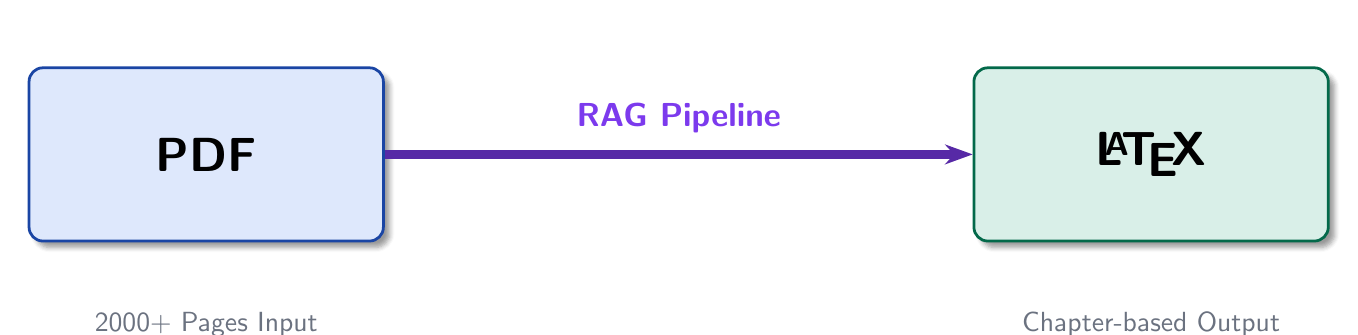
\begin{tikzpicture}[scale=1.2]
        % Central logo/icon representation
        \node[component=primary, minimum width=4.5cm, minimum height=2.2cm, font=\LARGE\sffamily\bfseries] (pdf) at (0,0) {PDF};
        \node[component=accent, minimum width=4.5cm, minimum height=2.2cm, font=\LARGE\sffamily\bfseries] (tex) at (10,0) {\LaTeX};
        
        % Arrow with RAG label
        \draw[flow=secondary, line width=3pt] (pdf.east) -- node[above, font=\large\sffamily\bfseries, text=secondary, yshift=3pt] {RAG Pipeline} (tex.west);
        
        % Decorative elements
        \node[font=\normalsize\sffamily, text=neutral] at (0,-1.8) {2000+ Pages Input};
        \node[font=\normalsize\sffamily, text=neutral] at (10,-1.8) {Chapter-based Output};
    \end{tikzpicture}
    
    \vspace{3cm}
    
    \begin{tabular}{rl}
        \textbf{\large Version:} & \large 1.0.0 \\[0.3cm]
        \textbf{\large Date:} & \large January 2026 \\[0.3cm]
        \textbf{\large Status:} & \large Planning Phase \\[0.3cm]
        \textbf{\large LLM Provider:} & \large Hugging Face Cloud \\
    \end{tabular}
    
    \vfill
    
    {\large\sffamily\color{neutral} High-Performance PDF to \LaTeX\ Conversion with Retrieval-Augmented Generation\par}
    
    \vspace{1cm}
\end{titlepage}

% ----------------------------------------------------------------------------
% TABLE OF CONTENTS
% ----------------------------------------------------------------------------
\tableofcontents
\newpage

% ============================================================================
% SECTION 1: SYSTEM OVERVIEW
% ============================================================================
\section{System Overview}

\begin{multicols}{2}

\subsection{Purpose}

PDF2TeX is a high-performance module designed to convert large PDF documents (2000+ pages) into structured \LaTeX\ files using Retrieval-Augmented Generation (RAG). The system prioritizes mathematical content accuracy and produces one \texttt{.tex} file per chapter.

\subsection{Key Objectives}

\begin{table}[H]
    \centering
    \caption{System Objectives and Targets}
    \begin{tabular}{@{}lll@{}}
        \toprule
        \textbf{Objective} & \textbf{Target} & \textbf{Priority} \\
        \midrule
        Processing Speed & $<$ 90 min / 2000 pg & High \\
        Math Accuracy & $>$ 95\% fidelity & Critical \\
        Output Quality & Compilable \LaTeX & Critical \\
        Scalability & 10+ concurrent docs & Medium \\
        \bottomrule
    \end{tabular}
\end{table}

\columnbreak

\subsection{Design Principles}

\begin{itemize}[leftmargin=*, itemsep=0.5em]
    \item \textbf{Modularity \& Separation of Concerns}\\
    Independent layers with clear responsibilities
    \item \textbf{Scalability}\\
    Ray-based distributed processing with horizontal scaling
    \item \textbf{Security by Design}\\
    Input validation, sandboxed compilation
    \item \textbf{Simplicity}\\
    Clear interfaces, minimal dependencies per module
    \item \textbf{Flexibility}\\
    Provider-agnostic LLM layer, pluggable backends
\end{itemize}

\end{multicols}

% ============================================================================
% SECTION 2: HIGH-LEVEL ARCHITECTURE
% ============================================================================
\newpage
\section{High-Level Architecture}

\subsection{System Context Diagram}

\begin{figure}[H]
    \centering
    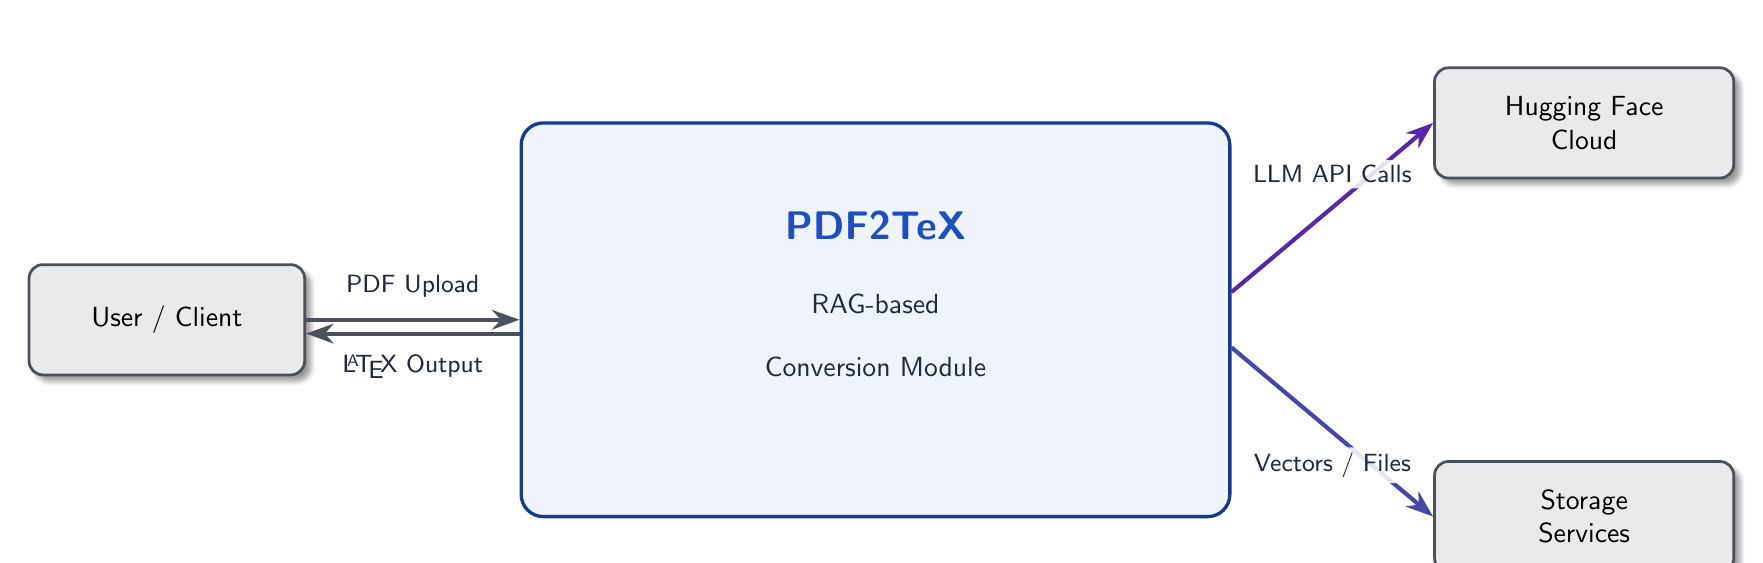
\begin{tikzpicture}[node distance=2cm and 3cm]
        
        % External actors
        \node[component=neutral, minimum width=3.5cm] (user) at (0, 0) {User / Client};
        \node[component=neutral, minimum width=3.8cm] (hf) at (18, 2.5) {Hugging Face\\Cloud};
        \node[component=neutral, minimum width=3.8cm] (storage) at (18, -2.5) {Storage\\Services};
        
        % Main system
        \node[container=primary, minimum width=9cm, minimum height=5cm] (system) at (9, 0) {};
        \node[font=\Large\sffamily\bfseries, text=primary!80!black] at (9, 1.2) {PDF2TeX};
        \node[font=\normalsize\sffamily, text=dark] at (9, 0.2) {RAG-based};
        \node[font=\normalsize\sffamily, text=dark] at (9, -0.6) {Conversion Module};
        
        % Connections with proper spacing
        \draw[flow=neutral, line width=1.5pt] (user.east) -- node[label text, pos=0.5, yshift=12pt] {PDF Upload} (system.west);
        \draw[flow=neutral, line width=1.5pt] ([yshift=-5pt]system.west) -- node[label text, pos=0.5, yshift=-12pt] {\LaTeX\ Output} ([yshift=-5pt]user.east);
        
        \draw[flow=secondary, line width=1.5pt] ([yshift=10pt]system.east) -- node[label text, pos=0.5, yshift=12pt] {LLM API Calls} (hf.west);
        \draw[flow=storage, line width=1.5pt] ([yshift=-10pt]system.east) -- node[label text, pos=0.5, yshift=-12pt] {Vectors / Files} (storage.west);
        
    \end{tikzpicture}
    \caption{System Context: PDF2TeX and External Dependencies}
\end{figure}

\vspace{1cm}

\subsection{Main Pipeline Flow}

\begin{figure}[H]
    \centering
    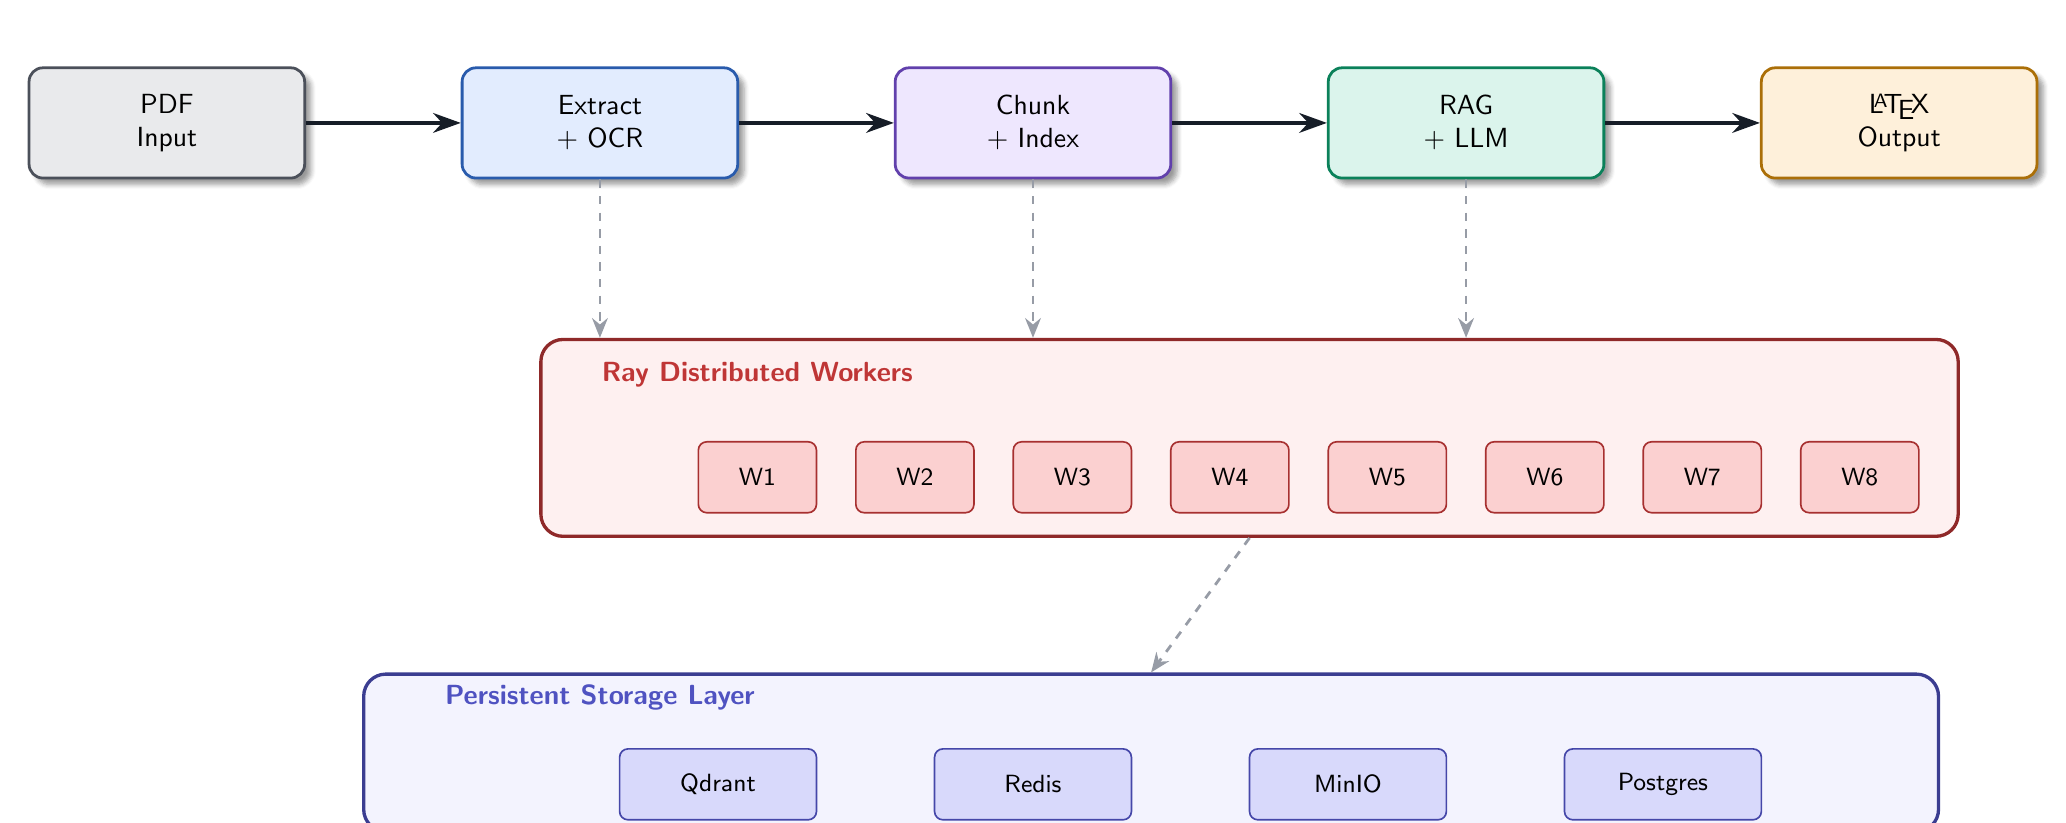
\begin{tikzpicture}[node distance=1.5cm and 2cm]
        
        % Pipeline stages with generous spacing
        \node[component=neutral, minimum width=3.5cm] (input) at (0, 0) {PDF\\Input};
        \node[component=extraction, minimum width=3.5cm] (extract) at (5.5, 0) {Extract\\+ OCR};
        \node[component=chunking, minimum width=3.5cm] (chunk) at (11, 0) {Chunk\\+ Index};
        \node[component=rag, minimum width=3.5cm] (rag) at (16.5, 0) {RAG\\+ LLM};
        \node[component=generation, minimum width=3.5cm] (output) at (22, 0) {\LaTeX\\Output};
        
        % Main flow arrows with labels
        \draw[flow=dark, line width=1.5pt] (input) -- (extract);
        \draw[flow=dark, line width=1.5pt] (extract) -- (chunk);
        \draw[flow=dark, line width=1.5pt] (chunk) -- (rag);
        \draw[flow=dark, line width=1.5pt] (rag) -- (output);
        
        % Worker pool
        \node[container=pipeline, minimum width=18cm, minimum height=2.5cm] (workers) at (13.75, -4) {};
        \node[font=\normalsize\sffamily\bfseries, text=pipeline!80!black] at (7.5, -3.2) {Ray Distributed Workers};
        
        % Individual workers with spacing
        \foreach \i in {1,...,8} {
            \node[worker=pipeline, minimum width=1.5cm] (w\i) at ({5.5 + \i * 2}, -4.5) {W\i};
        }
        
        % Connections to workers
        \draw[dataflow, line width=1pt] (extract.south) -- ++(0,-1.2) -| (workers.north -| extract);
        \draw[dataflow, line width=1pt] (chunk.south) -- ++(0,-1.2) -| (workers.north -| chunk);
        \draw[dataflow, line width=1pt] (rag.south) -- ++(0,-1.2) -| (workers.north -| rag);
        
        % Storage layer
        \node[container=storage, minimum width=20cm, minimum height=2cm] (storagelayer) at (12.5, -8) {};
        \node[font=\normalsize\sffamily\bfseries, text=storage!80!black] at (5.5, -7.3) {Persistent Storage Layer};
        
        \node[worker=storage, minimum width=2.5cm] (qdrant) at (7, -8.4) {Qdrant};
        \node[worker=storage, minimum width=2.5cm] (redis) at (11, -8.4) {Redis};
        \node[worker=storage, minimum width=2.5cm] (minio) at (15, -8.4) {MinIO};
        \node[worker=storage, minimum width=2.5cm] (pg) at (19, -8.4) {Postgres};
        
        % Storage connections
        \draw[dataflow, line width=1pt] (workers.south) -- (storagelayer.north);
        
    \end{tikzpicture}
    \caption{Main Processing Pipeline with Distributed Workers and Storage}
\end{figure}

% ============================================================================
% SECTION 3: COMPONENT ARCHITECTURE
% ============================================================================
\newpage
\section{Component Architecture}

\subsection{Extraction Layer}

\begin{figure}[H]
    \centering
    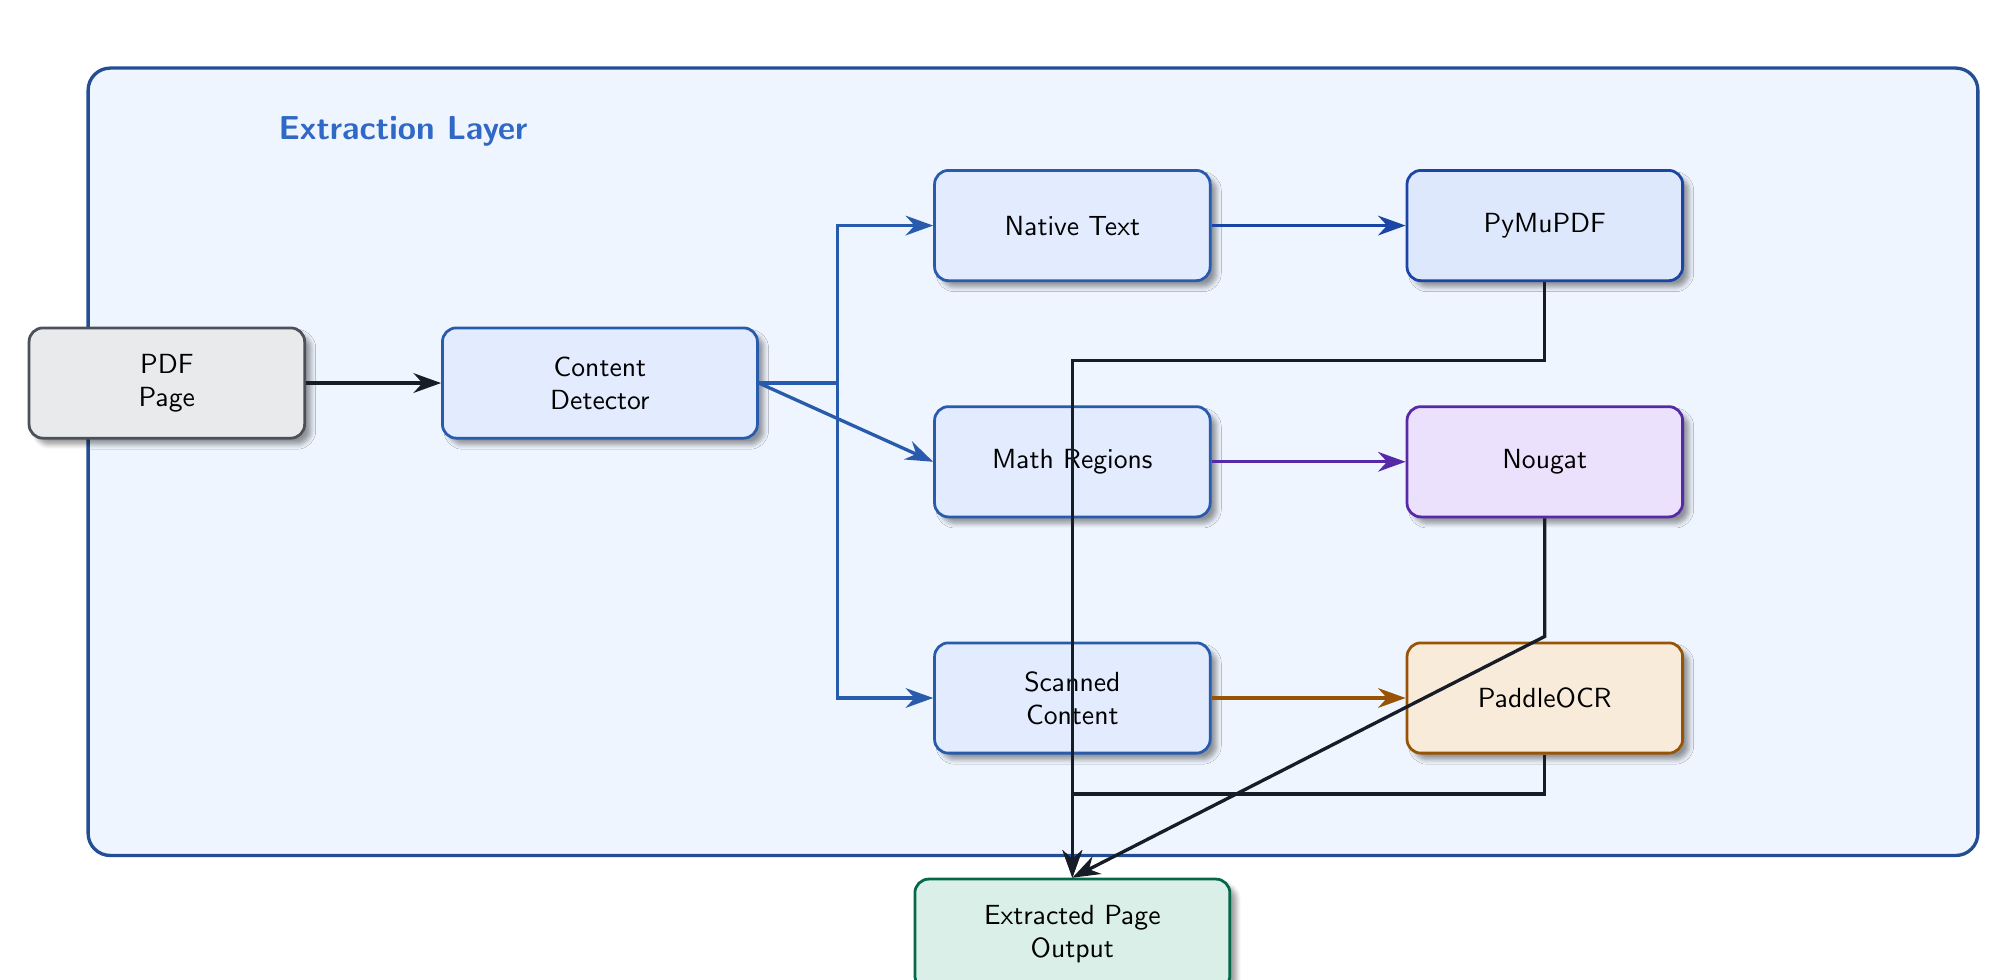
\begin{tikzpicture}[node distance=1cm and 2cm]
        
        % Container
        \node[container=extraction, minimum width=24cm, minimum height=10cm] (cont) at (12, -3) {};
        \node[section title, text=extraction!80!black] at (4, 1.2) {Extraction Layer};
        
        % Input
        \node[component=neutral, minimum width=3.5cm] (pdf) at (1, -2) {PDF\\Page};
        
        % Detection
        \node[component=extraction, minimum width=4cm] (detect) at (6.5, -2) {Content\\Detector};
        
        % Routers - spread vertically
        \node[component=extraction, minimum width=3.5cm] (text) at (12.5, 0) {Native Text};
        \node[component=extraction, minimum width=3.5cm] (math) at (12.5, -3) {Math Regions};
        \node[component=extraction, minimum width=3.5cm] (scan) at (12.5, -6) {Scanned\\Content};
        
        % Processors
        \node[component=primary, minimum width=3.5cm] (pymupdf) at (18.5, 0) {PyMuPDF};
        \node[component=secondary, minimum width=3.5cm] (nougat) at (18.5, -3) {Nougat};
        \node[component=warning, minimum width=3.5cm] (paddle) at (18.5, -6) {PaddleOCR};
        
        % Output aggregator
        \node[component=accent, minimum width=4cm] (agg) at (12.5, -9) {Extracted Page\\Output};
        
        % Connections with proper routing
        \draw[flow=dark, line width=1.2pt] (pdf) -- (detect);
        
        \draw[flow=extraction, line width=1.2pt] (detect.east) -- ++(1,0) |- (text.west);
        \draw[flow=extraction, line width=1.2pt] (detect.east) -- (math.west);
        \draw[flow=extraction, line width=1.2pt] (detect.east) -- ++(1,0) |- (scan.west);
        
        \draw[flow=primary, line width=1.2pt] (text) -- (pymupdf);
        \draw[flow=secondary, line width=1.2pt] (math) -- (nougat);
        \draw[flow=warning, line width=1.2pt] (scan) -- (paddle);
        
        \draw[flow=dark, line width=1.2pt] (pymupdf.south) -- ++(0,-1) -| (agg.north);
        \draw[flow=dark, line width=1.2pt] (nougat.south) -- ++(0,-1.5) -- (agg.north);
        \draw[flow=dark, line width=1.2pt] (paddle.south) -- ++(0,-0.5) -| (agg.north);
        
    \end{tikzpicture}
    \caption{Extraction Layer: Multi-path Content Processing}
\end{figure}

\vspace{0.5cm}

\begin{multicols}{2}
\subsubsection{Technology Stack}

\begin{table}[H]
    \centering
    \caption{Extraction Layer Technologies}
    \begin{tabular}{@{}llp{5cm}@{}}
        \toprule
        \textbf{Component} & \textbf{Tool} & \textbf{Purpose} \\
        \midrule
        Primary Parser & PyMuPDF & Fast native PDF extraction \\
        Math Extraction & Nougat & Neural PDF-to-\LaTeX \\
        Complex Layouts & Marker & ML structure detection \\
        OCR Engine & PaddleOCR & Scanned page OCR \\
        \bottomrule
    \end{tabular}
\end{table}

\columnbreak

\subsubsection{Processing Flow}
\begin{enumerate}[itemsep=0.3em]
    \item PDF page received from pipeline
    \item Content detector analyzes page type
    \item Routes to appropriate processor
    \item Results aggregated into unified format
    \item Output passed to chunking layer
\end{enumerate}

\end{multicols}

% ============================================================================
% MATH EXTRACTION
% ============================================================================
\newpage
\subsection{Math Extraction Pipeline}

\begin{figure}[H]
    \centering
    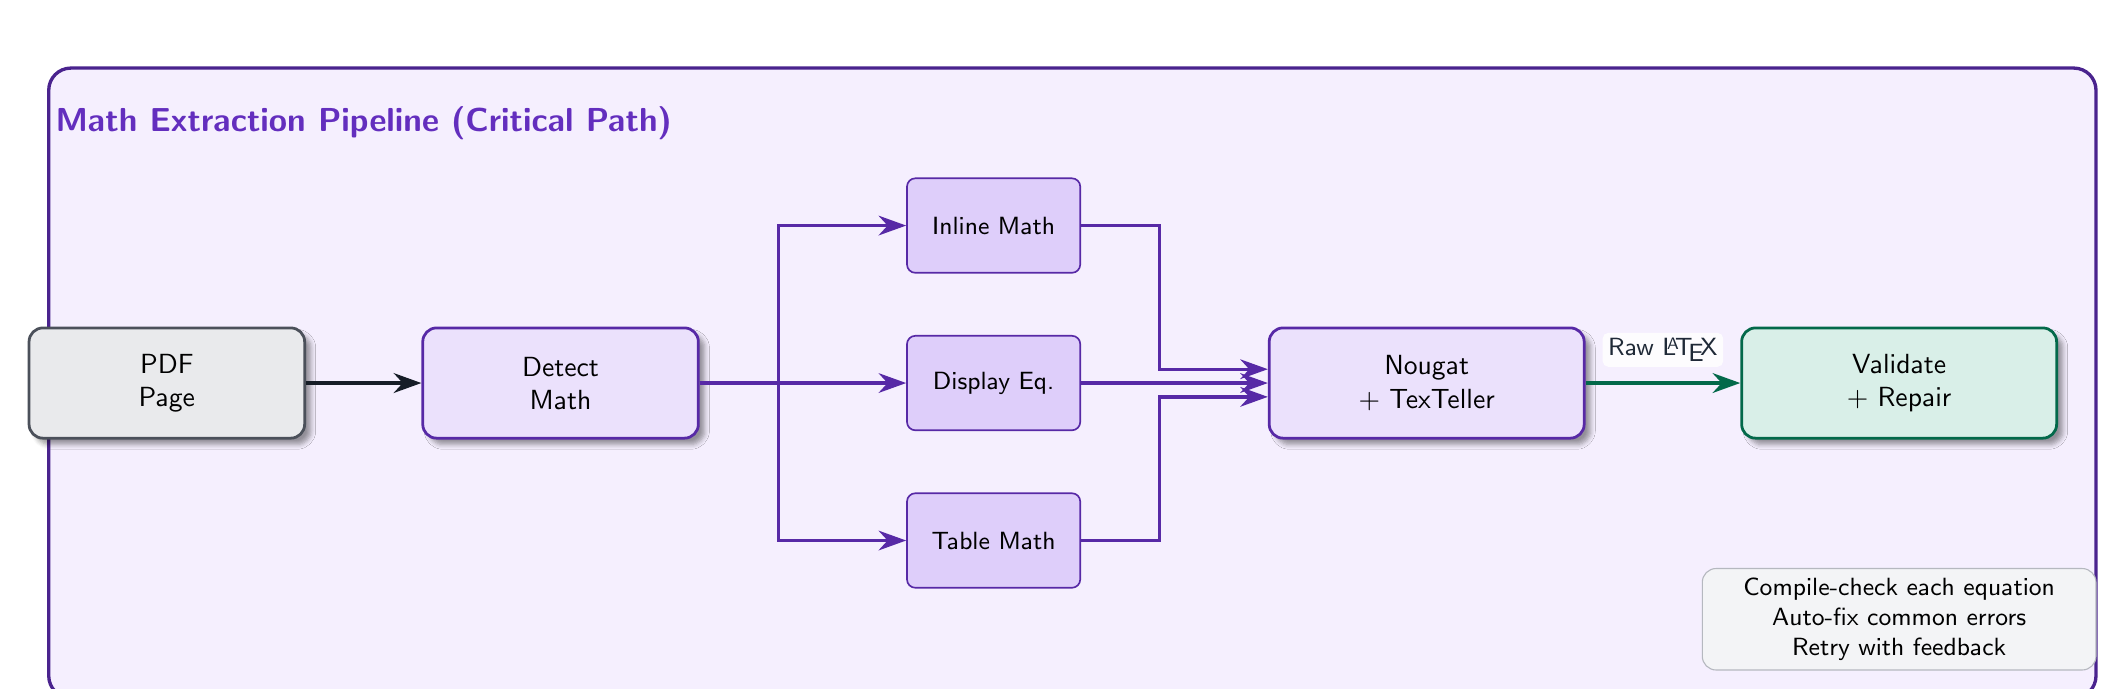
\begin{tikzpicture}[node distance=1.5cm and 2.5cm]
        
        % Container
        \node[container=secondary, minimum width=26cm, minimum height=8cm] (cont) at (13, -2.5) {};
        \node[section title, text=secondary!80!black] at (4, 0.8) {Math Extraction Pipeline (Critical Path)};
        
        % Flow
        \node[component=neutral, minimum width=3.5cm] (page) at (1.5, -2.5) {PDF\\Page};
        \node[component=secondary, minimum width=3.5cm] (detect) at (6.5, -2.5) {Detect\\Math};
        
        % Math types - spread out
        \node[worker=secondary, minimum width=2.2cm, minimum height=1.2cm] (inline) at (12, -0.5) {Inline Math};
        \node[worker=secondary, minimum width=2.2cm, minimum height=1.2cm] (display) at (12, -2.5) {Display Eq.};
        \node[worker=secondary, minimum width=2.2cm, minimum height=1.2cm] (table) at (12, -4.5) {Table Math};
        
        % Processor
        \node[component=secondary, minimum width=4cm] (nougat) at (17.5, -2.5) {Nougat\\+ TexTeller};
        
        % Validator
        \node[component=accent, minimum width=4cm] (valid) at (23.5, -2.5) {Validate\\+ Repair};
        
        % Connections
        \draw[flow=dark, line width=1.5pt] (page) -- (detect);
        
        \draw[flow=secondary, line width=1.2pt] (detect.east) -- ++(1,0) |- (inline.west);
        \draw[flow=secondary, line width=1.2pt] (detect.east) -- (display.west);
        \draw[flow=secondary, line width=1.2pt] (detect.east) -- ++(1,0) |- (table.west);
        
        \draw[flow=secondary, line width=1.2pt] (inline.east) -- ++(1,0) |- ([yshift=5pt]nougat.west);
        \draw[flow=secondary, line width=1.2pt] (display.east) -- (nougat.west);
        \draw[flow=secondary, line width=1.2pt] (table.east) -- ++(1,0) |- ([yshift=-5pt]nougat.west);
        
        \draw[flow=accent, line width=1.5pt] (nougat) -- node[label text, pos=0.5, yshift=12pt] {Raw \LaTeX} (valid);
        
        % Note box
        \node[draw=neutral!50, fill=light, rounded corners=5pt, minimum width=5cm, align=center, font=\small\sffamily] at (23.5, -5.5) {Compile-check each equation\\Auto-fix common errors\\Retry with feedback};
        
    \end{tikzpicture}
    \caption{Mathematical Content Extraction with Validation Loop}
\end{figure}

\vspace{1cm}

\subsection{Chunking Layer}

\begin{figure}[H]
    \centering
    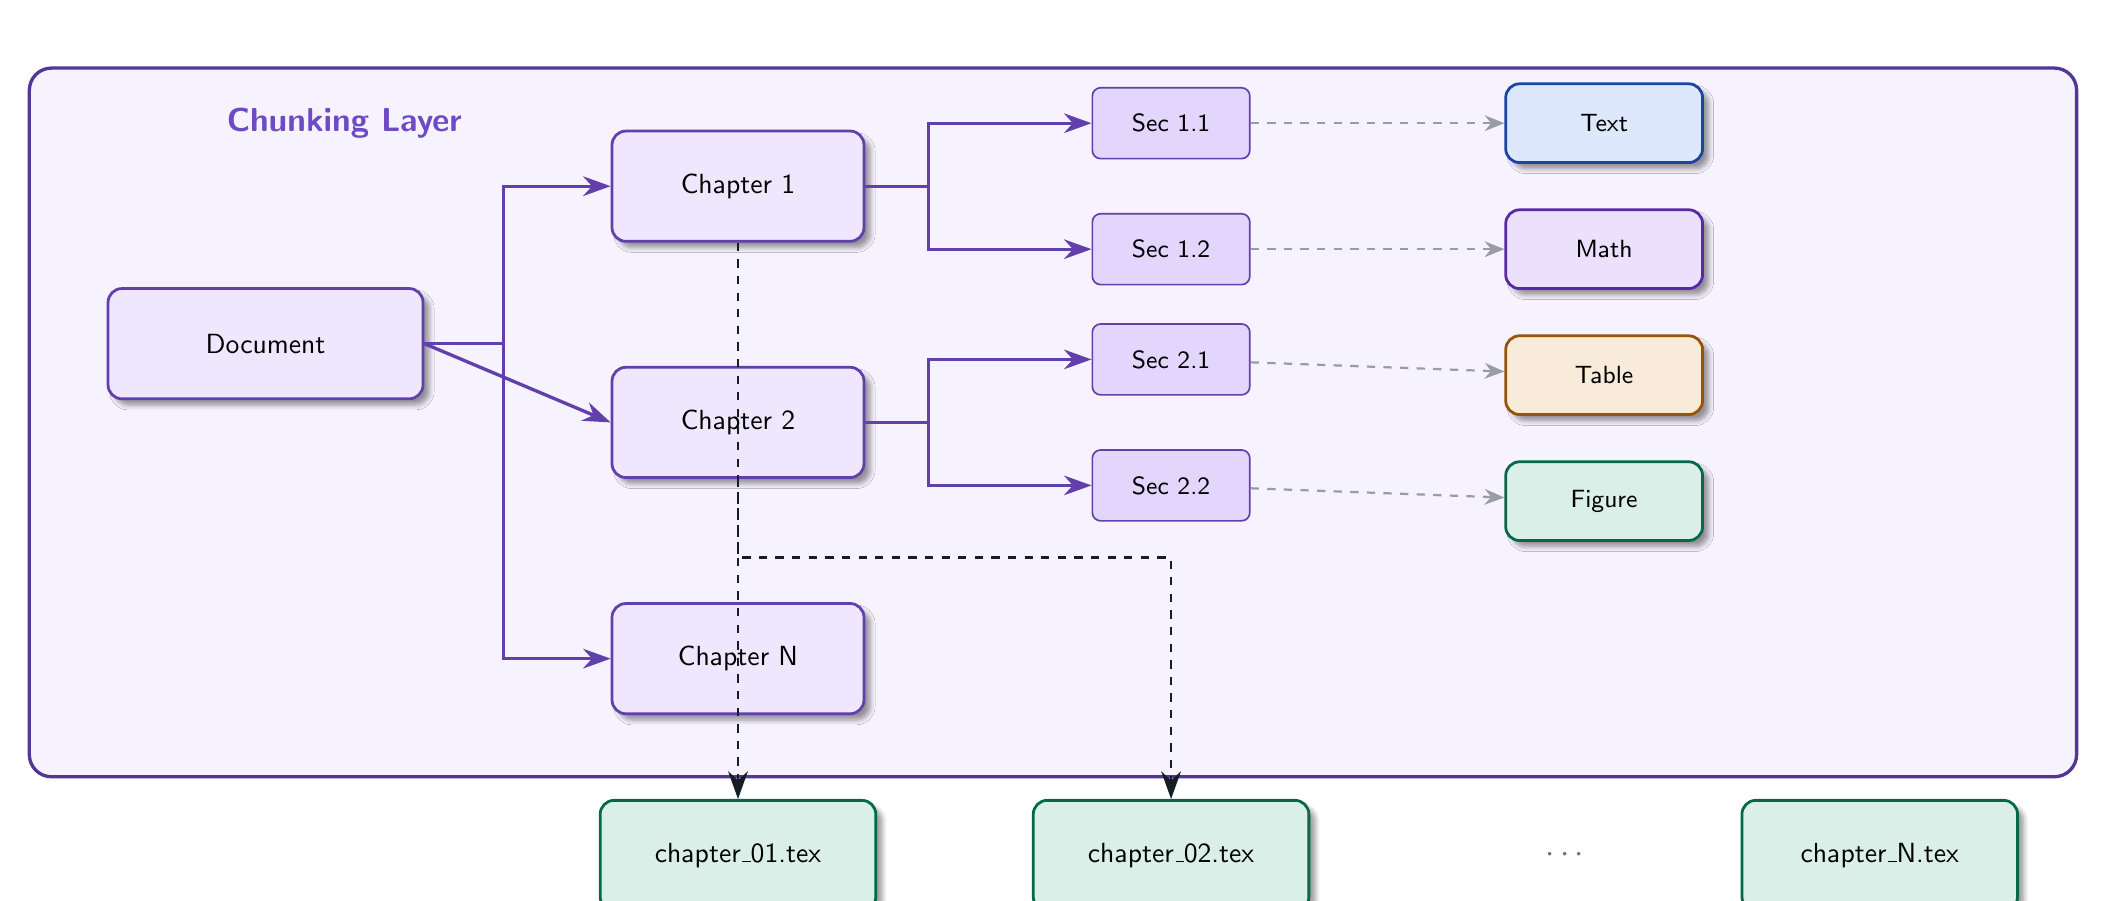
\begin{tikzpicture}[node distance=1cm and 2cm]
        
        % Container
        \node[container=chunking, minimum width=26cm, minimum height=9cm] (cont) at (13, -3) {};
        \node[section title, text=chunking!80!black] at (4, 0.8) {Chunking Layer};
        
        % Hierarchical structure
        \node[component=chunking, minimum width=4cm] (doc) at (3, -2) {Document};
        
        \node[component=chunking, minimum width=3.2cm] (ch1) at (9, 0) {Chapter 1};
        \node[component=chunking, minimum width=3.2cm] (ch2) at (9, -3) {Chapter 2};
        \node[component=chunking, minimum width=3.2cm] (chn) at (9, -6) {Chapter N};
        
        \node[worker=chunking, minimum width=2cm] (s11) at (14.5, 0.8) {Sec 1.1};
        \node[worker=chunking, minimum width=2cm] (s12) at (14.5, -0.8) {Sec 1.2};
        \node[worker=chunking, minimum width=2cm] (s21) at (14.5, -2.2) {Sec 2.1};
        \node[worker=chunking, minimum width=2cm] (s22) at (14.5, -3.8) {Sec 2.2};
        
        % Chunk types - well spaced
        \node[component=primary, minimum width=2.5cm, minimum height=1cm] (text) at (20, 0.8) {\small Text};
        \node[component=secondary, minimum width=2.5cm, minimum height=1cm] (math) at (20, -0.8) {\small Math};
        \node[component=warning, minimum width=2.5cm, minimum height=1cm] (tbl) at (20, -2.4) {\small Table};
        \node[component=accent, minimum width=2.5cm, minimum height=1cm] (fig) at (20, -4) {\small Figure};
        
        % Connections
        \draw[flow=chunking, line width=1.2pt] (doc.east) -- ++(1,0) |- (ch1.west);
        \draw[flow=chunking, line width=1.2pt] (doc.east) -- (ch2.west);
        \draw[flow=chunking, line width=1.2pt] (doc.east) -- ++(1,0) |- (chn.west);
        
        \draw[flow=chunking, line width=1pt] (ch1.east) -- ++(0.8,0) |- (s11.west);
        \draw[flow=chunking, line width=1pt] (ch1.east) -- ++(0.8,0) |- (s12.west);
        \draw[flow=chunking, line width=1pt] (ch2.east) -- ++(0.8,0) |- (s21.west);
        \draw[flow=chunking, line width=1pt] (ch2.east) -- ++(0.8,0) |- (s22.west);
        
        \draw[dataflow, line width=0.8pt] (s11) -- (text);
        \draw[dataflow, line width=0.8pt] (s12) -- (math);
        \draw[dataflow, line width=0.8pt] (s21) -- (tbl);
        \draw[dataflow, line width=0.8pt] (s22) -- (fig);
        
        % Output files
        \node[component=accent, minimum width=3.5cm] (out1) at (9, -8.5) {chapter\_01.tex};
        \node[component=accent, minimum width=3.5cm] (out2) at (14.5, -8.5) {chapter\_02.tex};
        \node[font=\large\sffamily, text=neutral] at (19.5, -8.5) {$\cdots$};
        \node[component=accent, minimum width=3.5cm] (outn) at (23.5, -8.5) {chapter\_N.tex};
        
        \draw[flow=dark, dashed, line width=1pt] (ch1.south) -- ++(0,-1) -| (out1.north);
        \draw[flow=dark, dashed, line width=1pt] (ch2.south) -- ++(0,-1) -| (out2.north);
        
    \end{tikzpicture}
    \caption{Hierarchical Chunking: Document $\rightarrow$ Chapter $\rightarrow$ Section $\rightarrow$ Typed Chunks}
\end{figure}

% ============================================================================
% RAG & GENERATION
% ============================================================================
\newpage
\subsection{RAG Layer}

\begin{figure}[H]
    \centering
    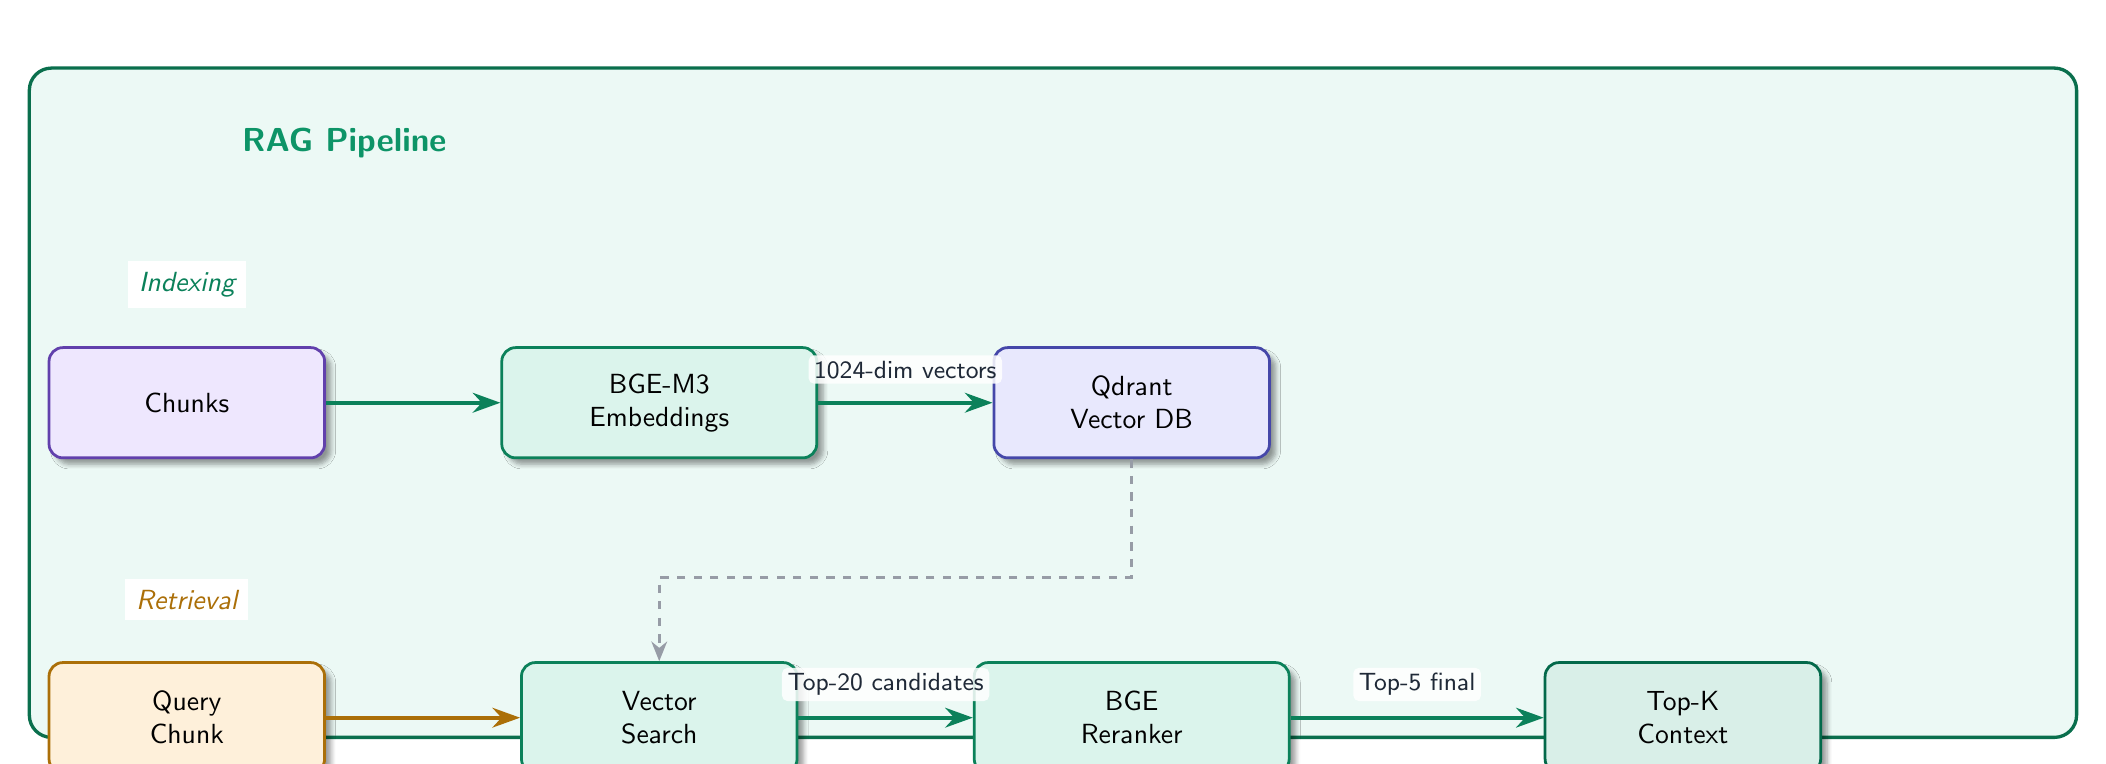
\begin{tikzpicture}[node distance=1.5cm and 3cm]
        
        % Container
        \node[container=rag, minimum width=26cm, minimum height=8.5cm] (cont) at (13, -2.5) {};
        \node[section title, text=rag!80!black] at (4, 0.8) {RAG Pipeline};
        
        % Indexing path label
        \node[font=\normalsize\sffamily\itshape, text=rag!70!black, fill=white, inner sep=4pt] at (2, -1) {Indexing};
        
        % Indexing path
        \node[component=chunking, minimum width=3.5cm] (chunks) at (2, -2.5) {Chunks};
        \node[component=rag, minimum width=4cm] (embed) at (8, -2.5) {BGE-M3\\Embeddings};
        \node[component=storage, minimum width=3.5cm] (qdrant) at (14, -2.5) {Qdrant\\Vector DB};
        
        % Retrieval path label
        \node[font=\normalsize\sffamily\itshape, text=generation!70!black, fill=white, inner sep=4pt] at (2, -5) {Retrieval};
        
        % Retrieval path
        \node[component=generation, minimum width=3.5cm] (query) at (2, -6.5) {Query\\Chunk};
        \node[component=rag, minimum width=3.5cm] (search) at (8, -6.5) {Vector\\Search};
        \node[component=rag, minimum width=4cm] (rerank) at (14, -6.5) {BGE\\Reranker};
        \node[component=accent, minimum width=3.5cm] (context) at (21, -6.5) {Top-K\\Context};
        
        % Connections with labels
        \draw[flow=rag, line width=1.5pt] (chunks) -- (embed);
        \draw[flow=rag, line width=1.5pt] (embed) -- node[label text, pos=0.5, yshift=12pt] {1024-dim vectors} (qdrant);
        
        \draw[flow=generation, line width=1.5pt] (query) -- (search);
        \draw[flow=rag, line width=1.5pt] (search) -- node[label text, pos=0.5, yshift=12pt] {Top-20 candidates} (rerank);
        \draw[flow=rag, line width=1.5pt] (rerank) -- node[label text, pos=0.5, yshift=12pt] {Top-5 final} (context);
        
        % Qdrant to search connection
        \draw[dataflow, line width=1pt] (qdrant.south) -- ++(0,-1.5) -| (search.north);
        
    \end{tikzpicture}
    \caption{RAG Pipeline: Parallel Indexing and Retrieval with Cross-Encoder Reranking}
\end{figure}

\vspace{0.8cm}

\subsection{Generation Layer}

\begin{figure}[H]
    \centering
    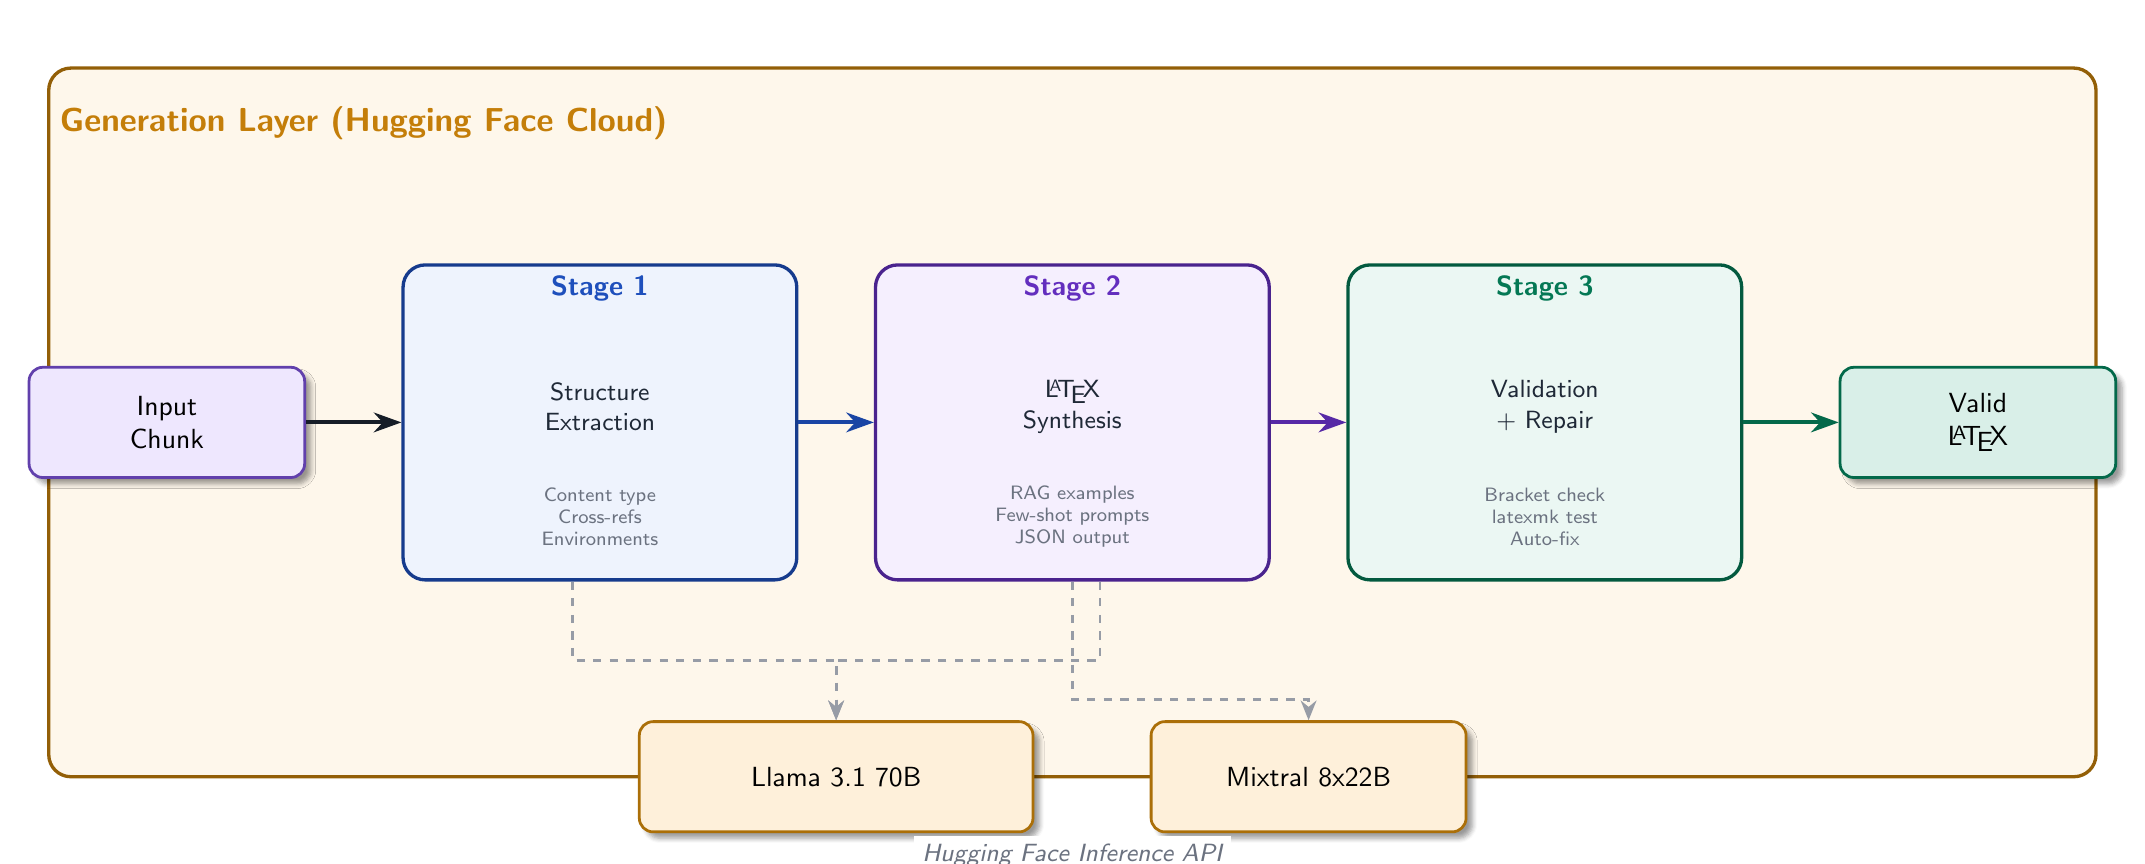
\begin{tikzpicture}[node distance=1cm and 1.5cm]
        
        % Container
        \node[container=generation, minimum width=26cm, minimum height=9cm] (cont) at (13, -3) {};
        \node[section title, text=generation!80!black] at (4, 0.8) {Generation Layer (Hugging Face Cloud)};
        
        % Input
        \node[component=chunking, minimum width=3.5cm] (input) at (1.5, -3) {Input\\Chunk};
        
        % Stage 1
        \node[container=primary, minimum width=5cm, minimum height=4cm] (s1) at (7, -3) {};
        \node[font=\normalsize\sffamily\bfseries, text=primary!80!black] at (7, -1.3) {Stage 1};
        \node[font=\small\sffamily, text=dark, align=center] at (7, -2.8) {Structure\\Extraction};
        \node[font=\scriptsize\sffamily, text=neutral, align=center] at (7, -4.2) {Content type\\Cross-refs\\Environments};
        
        % Stage 2
        \node[container=secondary, minimum width=5cm, minimum height=4cm] (s2) at (13, -3) {};
        \node[font=\normalsize\sffamily\bfseries, text=secondary!80!black] at (13, -1.3) {Stage 2};
        \node[font=\small\sffamily, text=dark, align=center] at (13, -2.8) {\LaTeX\\Synthesis};
        \node[font=\scriptsize\sffamily, text=neutral, align=center] at (13, -4.2) {RAG examples\\Few-shot prompts\\JSON output};
        
        % Stage 3
        \node[container=accent, minimum width=5cm, minimum height=4cm] (s3) at (19, -3) {};
        \node[font=\normalsize\sffamily\bfseries, text=accent!80!black] at (19, -1.3) {Stage 3};
        \node[font=\small\sffamily, text=dark, align=center] at (19, -2.8) {Validation\\+ Repair};
        \node[font=\scriptsize\sffamily, text=neutral, align=center] at (19, -4.2) {Bracket check\\latexmk test\\Auto-fix};
        
        % Output
        \node[component=accent, minimum width=3.5cm] (out) at (24.5, -3) {Valid\\\LaTeX};
        
        % LLM providers
        \node[component=generation, minimum width=5cm] (llama) at (10, -7.5) {Llama 3.1 70B};
        \node[component=generation, minimum width=4cm] (mixtral) at (16, -7.5) {Mixtral 8x22B};
        
        % Connections
        \draw[flow=dark, line width=1.5pt] (input) -- (s1);
        \draw[flow=primary, line width=1.5pt] (s1) -- (s2);
        \draw[flow=secondary, line width=1.5pt] (s2) -- (s3);
        \draw[flow=accent, line width=1.5pt] (s3) -- (out);
        
        \draw[dataflow, line width=1pt] ([xshift=-10pt]s1.south) -- ++(0,-1) -| (llama.north);
        \draw[dataflow, line width=1pt] ([xshift=10pt]s2.south) -- ++(0,-1) -| (llama.north);
        \draw[dataflow, line width=1pt] (s2.south) -- ++(0,-1.5) -| (mixtral.north);
        
        % HF label
        \node[font=\small\sffamily\itshape, text=neutral, fill=white, inner sep=3pt] at (13, -8.5) {Hugging Face Inference API};
        
    \end{tikzpicture}
    \caption{Three-Stage \LaTeX\ Generation with Validation Loop}
\end{figure}

% ============================================================================
% SECTION 4: PARALLEL PROCESSING
% ============================================================================
\newpage
\section{Parallel Processing Architecture}

\subsection{Ray Worker Distribution}

\begin{figure}[H]
    \centering
    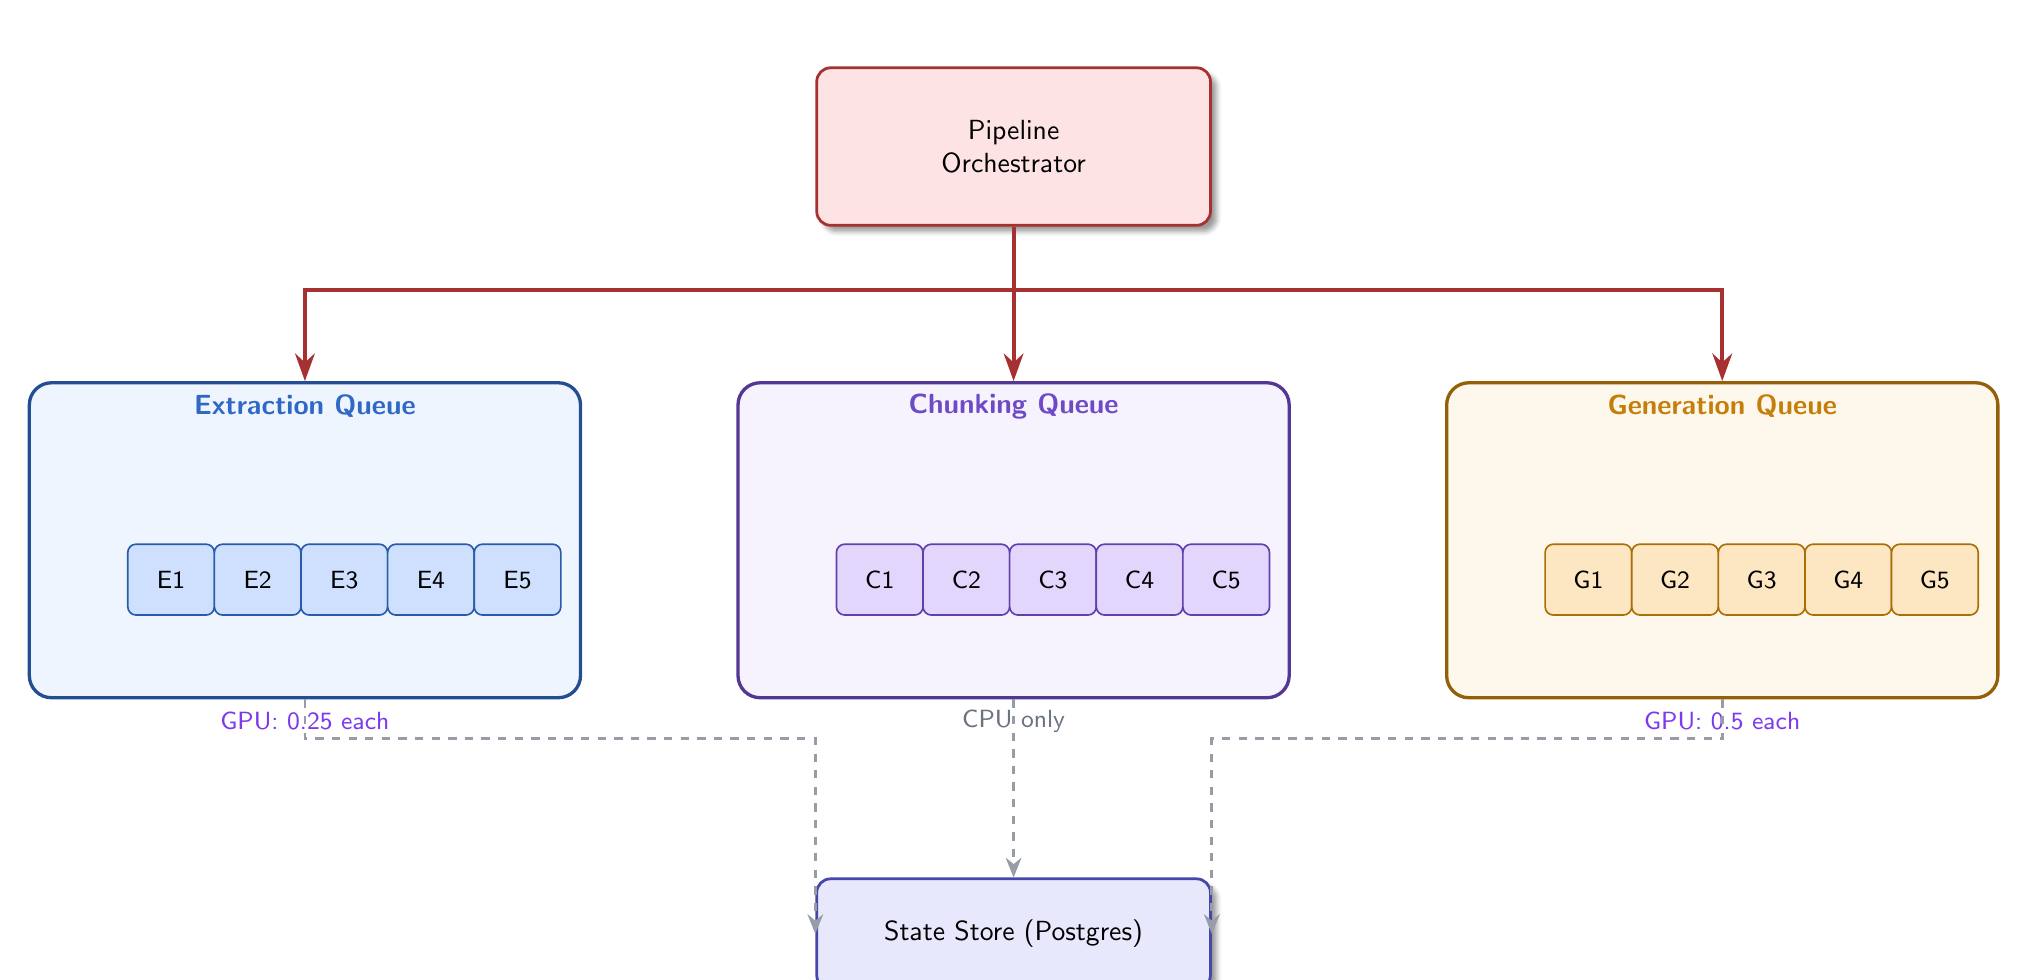
\begin{tikzpicture}[node distance=1cm and 2cm]
        
        % Orchestrator
        \node[component=pipeline, minimum width=5cm, minimum height=2cm] (orch) at (13, 2) {Pipeline\\Orchestrator};
        
        % Task queues - well spaced
        \node[container=extraction, minimum width=7cm, minimum height=4cm] (eq) at (4, -3) {};
        \node[font=\normalsize\sffamily\bfseries, text=extraction!80!black] at (4, -1.3) {Extraction Queue};
        \foreach \i in {1,...,5} {
            \node[worker=extraction, minimum width=1.1cm] at ({1.2 + \i * 1.1}, -3.5) {E\i};
        }
        \node[font=\small\sffamily, text=secondary] at (4, -5.3) {GPU: 0.25 each};
        
        \node[container=chunking, minimum width=7cm, minimum height=4cm] (cq) at (13, -3) {};
        \node[font=\normalsize\sffamily\bfseries, text=chunking!80!black] at (13, -1.3) {Chunking Queue};
        \foreach \i in {1,...,5} {
            \node[worker=chunking, minimum width=1.1cm] at ({10.2 + \i * 1.1}, -3.5) {C\i};
        }
        \node[font=\small\sffamily, text=neutral] at (13, -5.3) {CPU only};
        
        \node[container=generation, minimum width=7cm, minimum height=4cm] (gq) at (22, -3) {};
        \node[font=\normalsize\sffamily\bfseries, text=generation!80!black] at (22, -1.3) {Generation Queue};
        \foreach \i in {1,...,5} {
            \node[worker=generation, minimum width=1.1cm] at ({19.2 + \i * 1.1}, -3.5) {G\i};
        }
        \node[font=\small\sffamily, text=secondary] at (22, -5.3) {GPU: 0.5 each};
        
        % Connections
        \draw[flow=pipeline, line width=1.5pt] (orch.south) -- ++(0,-0.8) -| (eq.north);
        \draw[flow=pipeline, line width=1.5pt] (orch.south) -- (cq.north);
        \draw[flow=pipeline, line width=1.5pt] (orch.south) -- ++(0,-0.8) -| (gq.north);
        
        % State store
        \node[component=storage, minimum width=5cm] (state) at (13, -8) {State Store (Postgres)};
        \draw[dataflow, line width=1pt] (eq.south) -- ++(0,-0.5) -| (state.west);
        \draw[dataflow, line width=1pt] (cq.south) -- (state.north);
        \draw[dataflow, line width=1pt] (gq.south) -- ++(0,-0.5) -| (state.east);
        
    \end{tikzpicture}
    \caption{Ray Worker Pool Distribution by Task Type with GPU Allocation}
\end{figure}

\vspace{0.5cm}

\begin{multicols}{2}

\subsection{Performance Estimates}

\begin{table}[H]
    \centering
    \caption{Processing Time for 2000-Page Document}
    \begin{tabular}{@{}lrrr@{}}
        \toprule
        \textbf{Stage} & \textbf{Seq.} & \textbf{20 W} & \textbf{Limit} \\
        \midrule
        PDF Extraction & 30 min & 2 min & I/O \\
        Math (Nougat) & 4 hr & 15 min & GPU \\
        OCR (if needed) & 6 hr & 20 min & GPU \\
        Embedding & 40 min & 3 min & GPU \\
        LLM Generation & 8 hr & 30 min & API \\
        Validation & 20 min & 2 min & CPU \\
        \midrule
        \textbf{Total} & \textbf{19 hr} & \textbf{72 min} & \\
        \bottomrule
    \end{tabular}
\end{table}

\columnbreak

\subsection{Chunking Configuration}

\begin{table}[H]
    \centering
    \caption{Chunking Strategy by Content Type}
    \begin{tabular}{@{}lll@{}}
        \toprule
        \textbf{Type} & \textbf{Strategy} & \textbf{Size} \\
        \midrule
        Body Text & Recursive split & 512 tok \\
        Equations & Preserve whole & Variable \\
        Tables & Atomic & Variable \\
        Figures & Caption ref & 256 tok \\
        Code & Preserve whole & Variable \\
        \bottomrule
    \end{tabular}
\end{table}

\end{multicols}

% ============================================================================
% SECTION 5: OUTPUT & DEPLOYMENT
% ============================================================================
\newpage
\section{Output Structure \& Deployment}

\begin{multicols}{2}

\subsection{File Organization}

\begin{figure}[H]
    \centering
    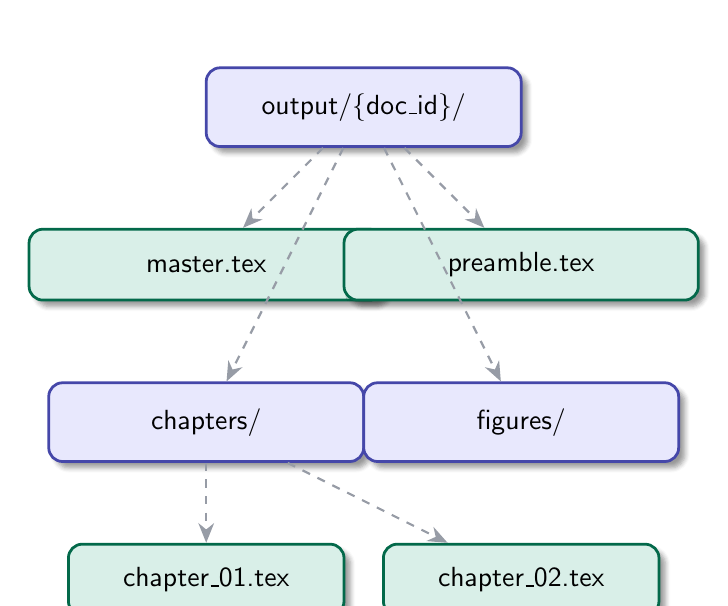
\begin{tikzpicture}[
        every node/.style={font=\normalsize\ttfamily},
        folder/.style={component=storage, minimum width=4cm, minimum height=1cm},
        file/.style={component=accent, minimum width=4.5cm, minimum height=0.9cm}
    ]
        % Root
        \node[folder] (root) at (0, 0) {output/\{doc\_id\}/};
        
        % Level 1
        \node[file] (master) at (-2, -2) {master.tex};
        \node[file] (preamble) at (2, -2) {preamble.tex};
        \node[folder] (chapters) at (-2, -4) {chapters/};
        \node[folder] (figures) at (2, -4) {figures/};
        
        % Chapter files
        \node[file, minimum width=3.5cm] (ch1) at (-2, -6) {chapter\_01.tex};
        \node[file, minimum width=3.5cm] (ch2) at (2, -6) {chapter\_02.tex};
        
        % Connections
        \draw[dataflow] (root) -- (master);
        \draw[dataflow] (root) -- (preamble);
        \draw[dataflow] (root) -- (chapters);
        \draw[dataflow] (root) -- (figures);
        \draw[dataflow] (chapters) -- (ch1);
        \draw[dataflow] (chapters) -- (ch2);
        
    \end{tikzpicture}
    \caption{Output Directory Structure}
\end{figure}

\subsection{Master Document}

\begin{verbatim}
% master.tex
\documentclass[11pt,a4paper]{book}
% Things to be included before \begin{document}, e.g. signature matrix, changelog, etc.

% Preparers shall be also included as reviewers in order to be notified (and sign) the release of the document.
\preparer{Mykhailo Dalchenko}{CTAO / Université de Genève - DPNC}

\reviewer{Mykhailo Dalchenko}{CTAO / Université de Genève - DPNC}
\reviewer{Maximillian Linhoff}{CTAO}

\approver{Mieke Bouwhuis}{CTAO}

% license / Copy Right
\setcopyright{\copyright{} CTAO / Université de Genève - DPNC \the\year}
\licence{\ccBySaNc}

% contributors list on second page, can be as many people as needed
\author{\ApplicationAuthor{}}{\ApplicationAuthorOrganization{}}{All Chapters}

\ChangeLogEntry{A}{001}{\today{}}{\ApplicationVersion}{}


\begin{document}
\frontmatter
\tableofcontents

\mainmatter
\input{chapters/chapter_01}
\input{chapters/chapter_02}
% ... auto-generated

\appendix
\input{chapters/appendix}

\backmatter
\bibliography{references}
\end{document}
\end{verbatim}

\columnbreak

\subsection{Deployment Architecture}

\begin{figure}[H]
    \centering
    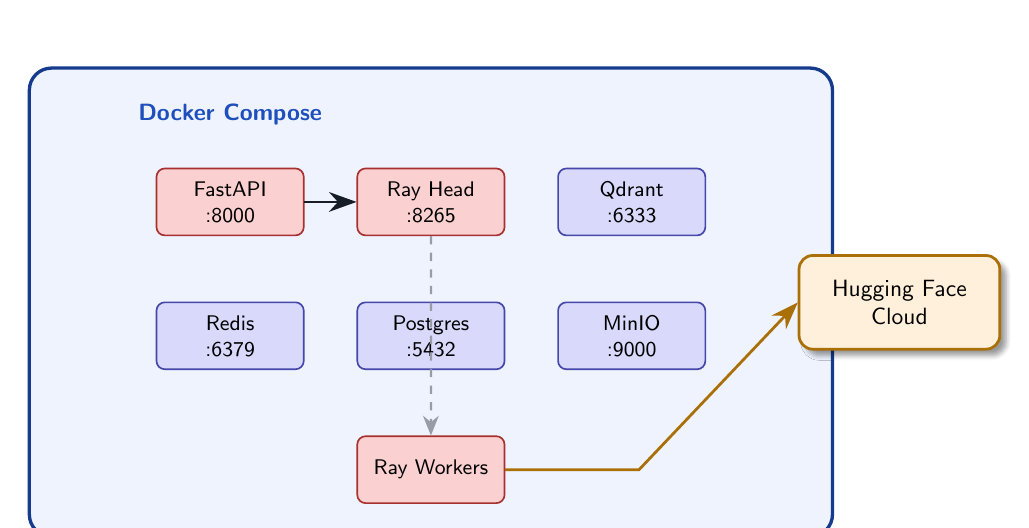
\begin{tikzpicture}[node distance=0.8cm and 1cm, scale=0.85, transform shape]
        
        % Docker container
        \node[container=primary, minimum width=12cm, minimum height=7cm] (docker) at (5, -2) {};
        \node[font=\normalsize\sffamily\bfseries, text=primary!80!black] at (2, 0.8) {Docker Compose};
        
        % Services row 1
        \node[worker=pipeline, minimum width=2.2cm, minimum height=1cm] (api) at (2, -0.5) {FastAPI\\:8000};
        \node[worker=pipeline, minimum width=2.2cm, minimum height=1cm] (ray) at (5, -0.5) {Ray Head\\:8265};
        \node[worker=storage, minimum width=2.2cm, minimum height=1cm] (qdrant) at (8, -0.5) {Qdrant\\:6333};
        
        % Services row 2
        \node[worker=storage, minimum width=2.2cm, minimum height=1cm] (redis) at (2, -2.5) {Redis\\:6379};
        \node[worker=storage, minimum width=2.2cm, minimum height=1cm] (pg) at (5, -2.5) {Postgres\\:5432};
        \node[worker=storage, minimum width=2.2cm, minimum height=1cm] (minio) at (8, -2.5) {MinIO\\:9000};
        
        % Workers
        \node[worker=pipeline, minimum width=2.2cm, minimum height=1cm] (worker) at (5, -4.5) {Ray Workers};
        
        % External
        \node[component=generation, minimum width=3cm] (hf) at (12, -2) {Hugging Face\\Cloud};
        
        % Connections
        \draw[flow=dark] (api) -- (ray);
        \draw[dataflow] (ray) -- (worker);
        \draw[flow=generation] (worker.east) -- ++(2,0) -- (hf.west);
        
    \end{tikzpicture}
    \caption{Docker Compose Deployment}
\end{figure}

\subsection{Hardware Requirements}

\begin{table}[H]
    \centering
    \caption{Resource Requirements}
    \begin{tabular}{@{}lll@{}}
        \toprule
        \textbf{Resource} & \textbf{Min} & \textbf{Rec.} \\
        \midrule
        CPU & 8 cores & 32 cores \\
        RAM & 32 GB & 64 GB \\
        GPU & 1× 3080 & 2× 4090 \\
        Storage & 100 GB & 500 GB \\
        \bottomrule
    \end{tabular}
\end{table}

\end{multicols}

% ============================================================================
% SECTION 6: DATA FLOW
% ============================================================================
\newpage
\section{End-to-End Data Flow}

\begin{figure}[H]
    \centering
    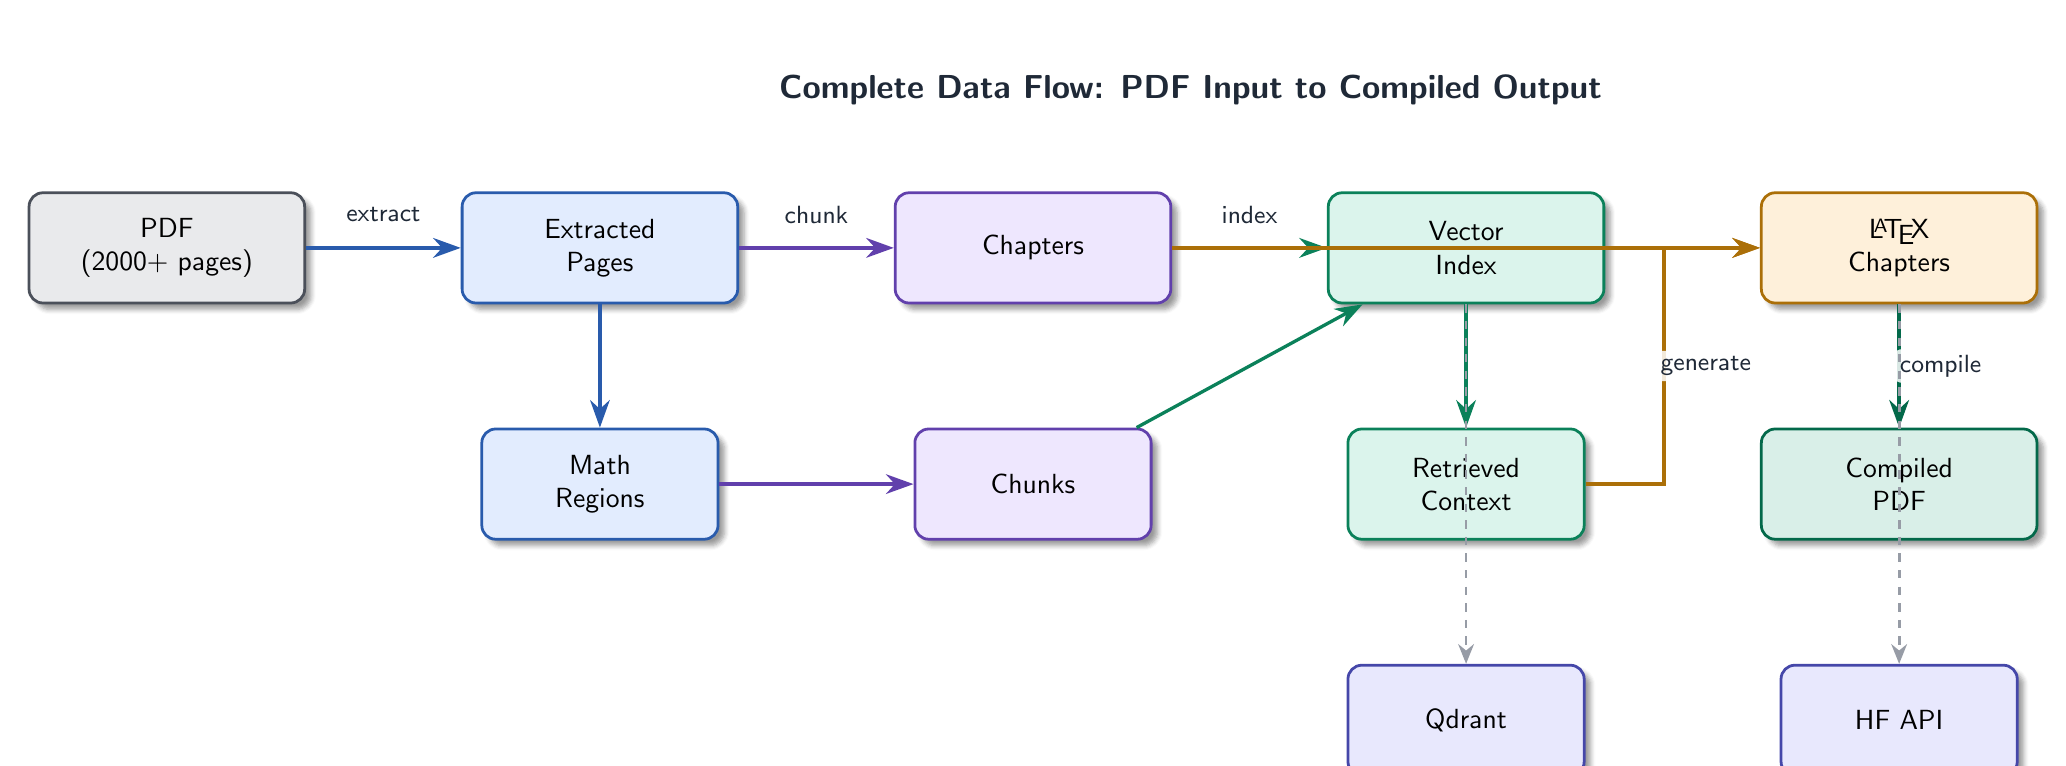
\begin{tikzpicture}[node distance=1.5cm and 2.5cm]
        
        % Title
        \node[section title] at (13, 2) {Complete Data Flow: PDF Input to Compiled Output};
        
        % Input
        \node[component=neutral, minimum width=3.5cm] (pdf) at (0, 0) {PDF\\(2000+ pages)};
        
        % Extraction outputs
        \node[component=extraction, minimum width=3.5cm] (pages) at (5.5, 0) {Extracted\\Pages};
        \node[component=extraction, minimum width=3cm] (math) at (5.5, -3) {Math\\Regions};
        
        % Chunking outputs
        \node[component=chunking, minimum width=3.5cm] (chapters) at (11, 0) {Chapters};
        \node[component=chunking, minimum width=3cm] (chunks) at (11, -3) {Chunks};
        
        % RAG
        \node[component=rag, minimum width=3.5cm] (vectors) at (16.5, 0) {Vector\\Index};
        \node[component=rag, minimum width=3cm] (context) at (16.5, -3) {Retrieved\\Context};
        
        % Generation
        \node[component=generation, minimum width=3.5cm] (latex) at (22, 0) {\LaTeX\\Chapters};
        
        % Final output
        \node[component=accent, minimum width=3.5cm] (output) at (22, -3) {Compiled\\PDF};
        
        % Flow with labels
        \draw[flow=extraction, line width=1.5pt] (pdf) -- node[label text, pos=0.5, yshift=12pt] {extract} (pages);
        \draw[flow=extraction, line width=1.2pt] (pages) -- (math);
        \draw[flow=chunking, line width=1.5pt] (pages) -- node[label text, pos=0.5, yshift=12pt] {chunk} (chapters);
        \draw[flow=chunking, line width=1.2pt] (math) -- (chunks);
        \draw[flow=rag, line width=1.5pt] (chapters) -- node[label text, pos=0.5, yshift=12pt] {index} (vectors);
        \draw[flow=rag, line width=1.2pt] (chunks) -- (vectors);
        \draw[flow=rag, line width=1.2pt] (vectors) -- (context);
        \draw[flow=generation, line width=1.5pt] (context.east) -- ++(1,0) |- node[label text, pos=0.25, xshift=15pt] {generate} (latex.west);
        \draw[flow=generation, line width=1.2pt] (chapters) -- (latex);
        \draw[flow=accent, line width=1.5pt] (latex) -- node[label text, pos=0.5, xshift=15pt] {compile} (output);
        
        % Data stores
        \node[component=storage, minimum width=3cm] (qdrant) at (16.5, -6) {Qdrant};
        \node[component=storage, minimum width=3cm] (hf) at (22, -6) {HF API};
        
        \draw[dataflow, line width=1pt] (vectors) -- (qdrant);
        \draw[dataflow, line width=1pt] (latex) -- (hf);
        
    \end{tikzpicture}
    \caption{Complete Data Flow from PDF Input to Compiled \LaTeX\ Output}
\end{figure}

\vspace{1cm}

% ============================================================================
% APPENDIX
% ============================================================================
\section{Technology Stack Summary}

\begin{multicols}{2}

\begin{table}[H]
    \centering
    \caption{Complete Technology Stack}
    \begin{tabular}{@{}lll@{}}
        \toprule
        \textbf{Layer} & \textbf{Technology} & \textbf{Version} \\
        \midrule
        \multirow{4}{*}{Extraction} & PyMuPDF & $\geq$ 1.24.0 \\
        & Nougat & $\geq$ 0.1.0 \\
        & PaddleOCR & $\geq$ 2.7.0 \\
        & Marker & Latest \\
        \midrule
        \multirow{2}{*}{Chunking} & LangChain & $\geq$ 0.2.0 \\
        & Custom splitters & -- \\
        \midrule
        \multirow{3}{*}{RAG} & Sentence-Trans. & $\geq$ 2.7.0 \\
        & Qdrant & $\geq$ 1.9.0 \\
        & BGE-M3 & Latest \\
        \bottomrule
    \end{tabular}
\end{table}

\columnbreak

\begin{table}[H]
    \centering
    \caption{Infrastructure Stack}
    \begin{tabular}{@{}lll@{}}
        \toprule
        \textbf{Layer} & \textbf{Technology} & \textbf{Version} \\
        \midrule
        \multirow{2}{*}{Generation} & HuggingFace Hub & $\geq$ 0.23.0 \\
        & Llama 3.1 70B & -- \\
        \midrule
        \multirow{2}{*}{Pipeline} & Ray & $\geq$ 2.20.0 \\
        & FastAPI & $\geq$ 0.111.0 \\
        \midrule
        \multirow{4}{*}{Infra} & PostgreSQL & 16 \\
        & Redis & 7 \\
        & MinIO & Latest \\
        & Docker & $\geq$ 24.0 \\
        \bottomrule
    \end{tabular}
\end{table}

\end{multicols}

% ============================================================================
% END DOCUMENT
% ============================================================================
\end{document}
